\section{Methodology}

\subsection{Task 1: propose a graph structure modeling methodology for recommender system}
It is challenging to develop effective data extraction and exploitation methods for Heterogeneous Information Network based recommender system.

\subsubsection*{Step 1: develop a generic graph structured data for recommendation problem}

Graph structure is being adopted in a wide range of applications. However, to our best of knowledge, none of them is taking a generic approach in forming the heterogeneous graph for recommender systems. HIN normally only optimized for a specific problem, and less adaptable to information evolution over time. 
Based on the nature of recommender system, we propose to accommodate not only user-item interaction, item features, and user profile information into the same heterogeneous information network. We also propose to further explore the semantic information by normalizing features on both item feature and user profile information into more atomic feature nodes. such practice would bring multiple benefits: 

\begin{itemize}
    
\item[1] Reduce data sparsity. By breaking up item features into more generic feature nodes would help increase the density of the network, and increase possible connectivity (mate-path) between nodes.

\item[2] With that, new in coming information would also transformed through the same decomposing process, hence making the graph structure adaptable to ever evolving changes.

\item[3] As the information graph cumulates auxiliary information in a holistic approach, suc structure also making problem context switch possible.

\end{itemize}

Of course, having a generic purpose HIN as training source introduce both complexity and noise. which we would discuss in Task 2 and Task 3.


\subsubsection*{Step 2: to develop transformation rule for the graph structure}

Recommendation test data sets are normally saved in csv format, which is quite different from the graph data structure we proposed above. Multi-Hub Network structure will be developed to transform the flat user-item data sets into a holistic feature-rich graph structure. Fig. \ref{fig:multihub}

\begin{figure*}[!t]
    \centering
    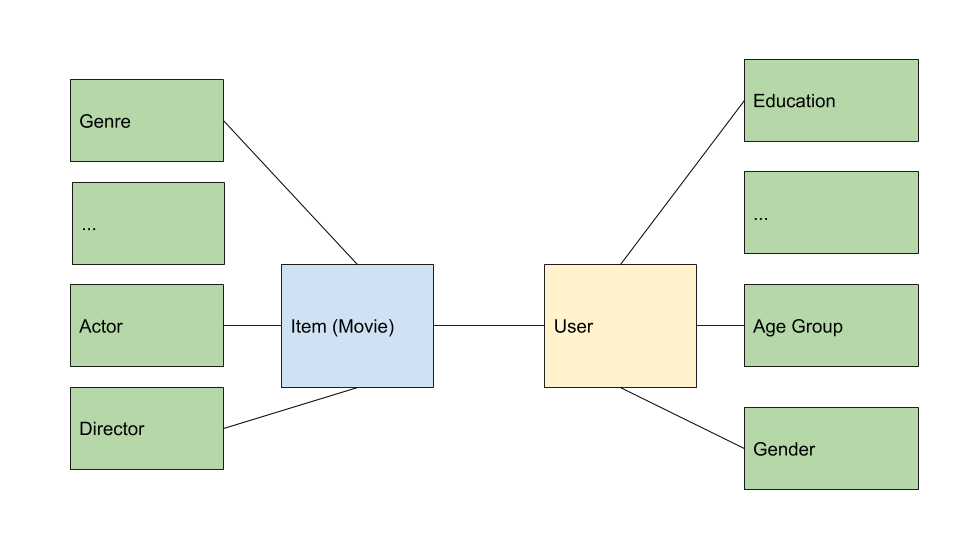
\includegraphics[width=0.8\textwidth]{figs/multi-hub.png}
    \caption{a multi-hub network structure based on Movielens data}\label{fig:multihub}
\end{figure*}


\subsection{Task 2: develop a comprehensive graph similarity measure}

Similarity measure the basis of many recommendation tasks, It evaluate the proximity among objects. Feature-based and link-based approaches are 2 main Similarity measures in HIN. 

The feature based approaches measure the similarity of objects based on their feature values, such as cosine similarity, Jaccard coefficient, and Euclidean distance. The link based approaches measure the similarity of objects based on their link structures in a graph. 

Similarity measure on HIN not only considers structure similarity of two objects but also takes the meta-path between two objects into account \citep{Shi2017}. \citet{Sun2011PathSim} propose PathSim that measure the semantics structure in meta-paths constituted by different-typed objects. The intuition for a single Meta-Path measure can be seen as: if source entity and target entity are exactly the same, then the round trip Meta-Paths $\mathcal{P}_1: A_1 \xrightarrow{r_1} A_2$ and 
$\mathcal{P}_1^{-1}: A_2 \xrightarrow{r_1^{-1}} A_1$ are always symmetric.

\theoremstyle{definition}
\begin{definition}[PathSim \cite{Sun2011PathSim}]\label{def:pathsim}
    Given a Meta-Path $\mathcal{P}$, PathSim between two entities $x$ and $y$ is:
    \begin{equation}
        sim(x,y)=\frac{2 \times \{|p_\text{x...y}:p_\text{y...x}| \in P\}}{\{|p_\text{x...x}:p_\text{x...x}| \in P\} + \{|p_\text{y...y}:p_\text{y...y}| \in P\}}
    \end{equation}
    where $x$ stands for source node, while $y$ for target node. 
    $x, y$ shares the same entity type $A_i$.
    $p_\text{x...y}$ stands for Meta-Path between entity $x$ and $y$. 
\end{definition}

HeteSim \citep{Shi2013HeteSim} proposed evaluate the relevance of any object pair under arbitrary meta-path. \citet{xiao2016avgsim} further improved HeteSim computation efficienc with AvgSim on large scale data.

For recommender systems, its a common use case for item-item and user-item recommendations based on similarity. Those measure is especially valuable when user-item interaction data is scarce, such as cold start problem. 

\subsection{Task 3: use embedding approach of large scale Information Network}

In recommendation settings, if we consider the graph structured HIN as a generic data repository. Such repository is not only capable of capture inter-relationship and semantic information between different types of data points (nodes). it is also adaptive to new information and grow the network organically. This allows HIN data repository capable contain rich information for complex recommendation problems. The challenge comes with a ever growing a graph network, is the noises increase alone with information cumulation.

Effective graph analytics provides users a deeper understanding of what is behind the data, and thus can benefit a lot of useful applications \citep{Cai2018}. Graph embedding is an effective yet efficient way to solve the graph analytics problem, while reduce the high computation and space cost, where the network structural information and graph properties are preserved into a low dimensional space.

Apart of overcoming computation constrains, embedding also play a important role of distilling relevant information, reducing noises for accordingly recommendation problem.

In order to learn effective heterogeneous network representations for summarizing important structural characteristics and properties of HINs. Based off work of DeepWalk \citep{perozzi2014deepwalk} and Node2Vec \citep{grover2016node2vec}, we characterize nodes from HINs with low-dimensional vectors, i.e., embeddings. 
Compared with meta-path based similarity, instead of relying on explicit path connection, embedding encode valuable feature data with latent vectors. The learned embeddings are in a more compact form that is easy to use and integrate. 
Motif-based approach \citep{tsourakakis2017scalable} and attention based approach \citep{Hu2018}, \citep{lee2018graph} yield effective results in both data mining and recommendation research filed.
Last but not least, embedding approach creates denser data, that make the recommender system being more resistant to noisy and sparse data. 

Followed by Task 2 similarity measure. In recommender system, we normally consider nodes proximity base on the weights of connecting edge between source and target nodes. As illustrated in GraRep \citep{cao2015grarep}. The model learns low dimensional vectors to represent vertices by integrates global structural information of the graph into the learning process.

On the other hand, GraphSAGE defined nodes proximity by comparing nodes' neighborhood. It introduced a general inductive framework to efficiently generate node embeddings for previously unseen data by leveraging node feature information. \citet{hamilton2017inductive} uses function that generates embeddings by sampling and aggregating features from a node’s local neighborhood.

Subsequently, fusion functions is used to integrate multiple node or meta-path embeddings into a single representation for recommendation. These fusion functions provide flexible ways to transform HIN embeddings into useful information for recommendation.


\subsection{Task 4: extend Heterogeneous Information Network to accommodate temporary information through time}

Most of the research mentioned above is based on static data. After defining suitable Similarity Measure (Task 2) and fitting Embedding Approach (Task 3) for the recommender system. In this task we would like to extend previous tasks to include temporal information, and data dynamics for our recommender system to taking account. \citet{he2014exploiting} extend the meta
path-based similarity measure PathSim by incorporating richer information, such as
transitive similarity and temporal dynamics. 

At the same time, in order to make HIN based recommender system to be time aware. Architecture adjustment is required accordingly. Graph Spatial-temporal Networks aim to learn unseen patterns from spatial-temporal graphs, which are increasingly important in many applications \citep{wu2019comprehensive}. 
The goal of graph spatial-temporal networks can be forecasting future node values or labels, or predicting spatial-temporal graph labels. Recent studies have explored the use of GCNs for action recognition \citep{yan2018spatial}, and GCNs in combination of with RNN \citep{li2017diffusion} or CNN \citep{yu2017spatio} in transportation traffic prediction.

So far GCNBased Graph Spatial-Temporal Networks have limited implementation in the recommender system. Based on the embedding methodology mentioned in Task 3, users and item nodes relationship can be treated as adjacency matrix, hence, user can be represented as a summation of K adjacency matrices of item-user edge. Subsequently, Graph Convolution can then applying different weights to its neighboring edges and sum them. By extending the temporal flow as graph edges, using a unified GCN model, spatial and temporal information can be extracted jointly.

\subsection{Task 5: develop recommendation framework based Heterogeneous Information Network}

Due to the flexibility in modelling data heterogeneity, HIN based recommendation adopts the model complex characterize and heterogeneous auxiliary data for recommender systems.

\subsubsection*{Step 1: HIN based recommendation on static data sets}
There are mainly 2 approaches in static data settings for performing recommendation tasks via HIN. 

Similarity base approach, which is mostly mentioned in task 2. The strength of similarity based approach are mostly comes down to computation efficiency. some of the approaches, such as PathSim \citep{Sun2011PathSim}, and AvgSim \citep{xiao2016avgsim} had been well researched and have a number mathematical optimization for recommender problem. however, latent structure features of users and items relationship are not fully used, when using path/node based similarity methods.

Alternatively, as mentioned in task 3, node embedding and meta-path embedding had been a rising research topic in recently years. Notables, \citet{shi2018heterogeneous} had proposed using node embeddings are first transformed by a set of fusion functions, and then extend the information into a matrix factorization (MF) model. The extended MF model together with fusion functions are jointly optimized for the rating prediction task.

\subsubsection*{Step 2: HIN based recommendation on dynamic temporal data sets}

In real-world settings, users interest is dynamic and influenced by the past experience. Temporal information is important for improving recommendations' accuracy. However due to the complexity of graph structure and computation restrictions. its a big challenge for reflecting both information into recommender system. Recent development in Graph Neural Network (GNN) and Attention Model had shown some exciting development in taking account of temporal information and user-item interaction sequences \citep{yu2017spatio}.  

There are two basic approaches currently exploring how to generalize CNNs to structured data forms: 
The First is to expand the spatial definition of a convolution \citep{niepert2016learning}. It rearranges the vertices into certain grid forms to perform convolution operations. The Second is to manipulate in the spectral domain with graph Fourier transforms \citep{bruna2013spectral}. Spectral graph convolution uses spectral framework to apply convolutions in spectral domains.

\citet{song2019session} propose a dynamic-graph-attention neural network based recommender system for online communities. \citet{Hu2018recommender} propose a unified model LGRec to fuse local and global information for top-N recommendation in HIN.


\subsection{Task 6:  A case study for validating the proposed recommendation approaches}

The research will be verified from two aspects: 

First, public datasets, such as DBLP DBLP Citation Networks, MovieLens data sets (http://www.grouplens.org/node/73), will be used to verify the effectiveness of the graph modeling approach for recommender system. Similarity measure as well as adaptability are the core parts of the approach, each aspects will be verified accordingly. 

Second, the approach will be used in a real world data sets. Real data sets from the tourism and real-estate industry will be used to further test the effectiveness of the method.

